\documentclass[t]{beamer}
\usetheme[deutsch]{KIT}
\setbeamercovered{transparent}
\setbeamertemplate{navigation symbols}{}

\KITfoot{Tutoriumsmaterial von Joachim Priesner, Sebastian Ullrich und Max Wagner \hspace{2.5cm} Basierend auf den Folien von Simon Stroh und Moritz v. Looz}
\usepackage[utf8]{inputenc}
\usepackage{amsmath}
\usepackage{ifthen}
\usepackage{amssymb}
\usepackage{tikz}
\usepackage{ngerman}
\usetikzlibrary{automata}
\usenavigationsymbols


\title{Theoretische Grundlagen der Informatik}
\subtitle{Tutorium}
\author{Moritz von Looz, Simon Stroh}

\institute[ITI]{Institut für Theoretische Informatik}

\TitleImage[height=\titleimageht]{images/tmaschine.png}

\newcommand{\N}{\ensuremath{\mathbb{N}}}
\newcommand{\M}{\ensuremath{\mathcal{M}}}
\newcommand{\classP}{\ensuremath{\mathcal{P}}}
\newcommand{\classNP}{\ensuremath{\mathcal{NP}}}
\newcommand{\co}{\ensuremath{\mathsf{co\text{-}}}}
\newcommand{\pot}{\ensuremath{\mathcal{P}}}
\newcommand{\abs}[1]{\ensuremath{\left\vert #1 \right\vert}}
\newcommand{\menge}[2]{\ensuremath{\left\lbrace #1 \,\middle\vert\, #2 \right\rbrace}}
\newcommand{\ducttape}[1]{\vspace{#1}}
\newcommand{\neglit}[1]{\overline{#1\vphantom{x^a}}}
\newcommand{\recipe}{\raisebox{-.3cm}{
\includegraphics[scale=.15]{images/chefs-cap.png}}\hspace{0.2cm}}

\newcommand{\invincible}{\setbeamercovered{invisible}} %  "Yesss! I am invincible!!" (Boris Grishenko)
\newcommand{\vincible}{\setbeamercovered{transparent}}

% \@ifundefined{tikzset}{}{\tikzset{initial text=}} % Text "start" bei Startknoten unterdrücken
\tikzstyle{every node}=[thick]
\tikzstyle{every line}=[thick]

\newcommand{\tutnr}[1]{
  \subtitle{Tutorium #1}
	\begin{frame}
		\maketitle
	\end{frame}
}

\newcommand{\uebnr}[1]{
  \subtitle{Anmerkungen zum #1. Übungsblatt}
	\begin{frame}
		\maketitle
	\end{frame}
}

\begin{document}

\tutnr{5}

\section{Wdh. Entscheidbarkeit}
\subsection{Wdh. Entscheidbarkeit}
\begin{frame}
	\frametitle{Aufgabe zur Entscheidbarkeit}
	
	Sei $L$ eine nicht entscheidbare Sprache \"uber dem Alphabet $\Sigma=\{0,1\}$ und sei $(01)^k \not\in L$ f\"ur jedes $k\in \mathbb N_{>0}$.
	
Zeige: Die Sprache \[L' = \{w_1\#w_2\mid (w_1 \in L \wedge w_2 \not\in L) \text{ oder } (w_1 \not\in L \wedge w_2 \in L) \}\]
\"uber dem Alphabet $\Sigma'=\{0, 1, \#\}$ ist nicht entscheidbar.

	\invincible \pause
	
	\ducttape{1cm}	
	
	\only<2-3>{
Annahme: $L'$ ist entscheidbar. Sei $M'$ dann eine Turingmaschine, die $L'$ entscheidet. $M'$ entscheidet also zun\"achst, ob der erste Teil des Wortes in $L$ liegt, und dann, ob der zweite Teil des Wortes nicht in $L$ liegt.

Sei $M$ eine Turingmaschine, die die erste Phase von $M'$ simuliert. Dann entscheidet $M$ die Sprache $L$, was ein Widerspruch zur Annahme ist.

	\pause
	\begin{center}
        \Huge{\textbf{\color{red}NOPE}}
    \end{center}
	
	}

	\only<4>{	
	Annahme: $L'$ ist entscheidbar. 
Sei $M'$ eine TM, die $L'$ entscheidet.
F\"ur ein Wort $w \in \Sigma^*$ konstruiere das Wort $w'=w\#01$. 
Dann gilt: $w' \in L' \Leftrightarrow w \in L$. 

Damit kann man $L$ wie folgt entscheiden, im Widerspruch zur Nichtentscheidbarkeit von $L$:\\
%F\"ur $w \in \Sigma^*$ konstruiere $w'=w\#01$.
Simuliere die TM $M'$ auf Eingabe $w'$ und akzeptiere $w \in L$ gdw. $M'$ $w' \in L'$ akzeptiert.
	}

	\vincible
	
\end{frame}

\section{Probleme}
\subsection{Probleme}
\begin{frame}
 \frametitle{Probleme}
 \begin{block}{Definition (Skript)}
 Ein \emph{Problem $\Pi$} ist gegeben durch:
 \begin{enumerate}
  \item eine allgemeine Beschreibung aller vorkommenden Parameter;
  \item eine genaue Beschreibung der Eigenschaften, welche die Lösung haben soll
 \end{enumerate}
 \end{block}
 Ein \emph{Problembeispiel} \textit{I} \emph{(Instanz)} von $\Pi$ erhalten wir, indem wir die Parameter von $\Pi$ festlegen.
\end{frame}

\begin{frame}
 \frametitle{Entscheidungsproblem}
 \begin{block}{Definition}
  Ein Entscheidungsproblem ist ein Problem, bei dem die Lösung "`Ja"' oder "`Nein"' lautet. 
  Entscheidungsprobleme lassen sich gut auf Sprachen abbilden.
 \end{block}
\end{frame}

\begin{frame}
 \frametitle{Optimierungsproblem und Entscheidungsproblem}
 \begin{block}{Beispiel}
  \begin{enumerate}
   \item Die Aufgabe, aus einem gegebenen Blech möglichst viele sternförmige Weihnachtsplätzchen zu gewinnen, ist ein Optimierungsproblem.
   \item Die Frage, ob aus diesem Blech mindestens $k$ Plätzchen gewonnen werden können, ist ein zugehöriges Entscheidungsproblem.
  \end{enumerate}
 \end{block}
 \begin{block}{Überlegung}
  Wie kann man mit einer Turingmaschine, welche das Entscheidungsproblem löst, das Optimierungsproblem lösen?
 \end{block}
 Hinweis: Nimm an, dass es nur endlich viele mögliche Kekskonfigurationen auf einem Backblech gibt.
\end{frame}

\begin{frame}
 \frametitle{Optimierungsproblem und Entscheidungsproblem}
 \begin{block}{Überlegung}
  Wie kann man mit einer Turingmaschine, welche das Entscheidungsproblem löst, das Optimierungsproblem lösen?
 \end{block}
\begin{block}{Strategie}
 \begin{enumerate}
  \item Zunächst mit binärer Suche das maximale $k$ herausfinden.
  \item Die $n$-te Formplatzierung beliebig festlegen. Wenn das Problem für $k-n$ Plätzchen noch lösbar ist, war die Platzierung richtig, sonst nimm sie zurück.
  \item Wiederhole Schritt 2, bis alle Formen platziert sind.
 \end{enumerate}
\end{block}
\end{frame}


%TODO: Grafik

\begin{frame}
 \frametitle{Entscheidungsproblem}
  Gegeben seien ein gerichteter Graph $G = (V, E)$ und zwei Knoten $v, w \in V$.
  
  \begin{enumerate}
  	\item Betrachte die Menge der Wege von $v$ nach $w$ in $G$ und formuliere ein naheliegendes Optimierungsproblem.
  	\item Formuliere ein zu deinem Optimierungsproblem gehörendes Optimalwertproblem.
  	\item Formuliere ein zu deinem Optimierungsproblem gehörendes Entscheidungsproblem.
  \end{enumerate}
\end{frame}

\subsection{Kodierungsschemata}
\begin{frame}
 \frametitle{Kodierungsschemata (VL)}
 \begin{block}{Definition Kodierungsschema}
 Ein \emph{Kodierungsschema} $s$ ordnet jeder Instanz eines Problems eine Zeichenkette oder Kodierung über einem Alphabet $\Sigma$ zu. 
 Die Eingabelänge eines Problembeispiels ist die Anzahl der Symbole seiner Kodierung.
 Dabei gibt es natürliche verschiedene Kodierungsschemata für ein bestimmtes Problem.
 \end{block}
 \begin{block}{Äquivalenz}
  Zwei Kodierungsschemata $s_1$, $s_2$ heißen \emph{äquivalent} bezüglich eines Problems $\Pi$, falls es Polynome $p_1$, $p_2$ gibt, sodass gilt:
  \[
   (|s_1(I)| = n \Rightarrow |s_2(I)| \leq p_2(n))\mbox{ und } (|s_2(I)| = m \Rightarrow |s_1(I)| \leq p_1(m))
  \]
für alle Problembeispiele I von $\Pi$.
 \end{block}
\end{frame}

\begin{frame}
 \frametitle{Kodierungsschemata}
 Das Entscheidungsproblem \textit{PRIMES} besteht darin, zu entscheiden, ob es sich bei einer gegebenen natürlichen Zahl $p>1$ um eine Primzahl handelt. 
Eine Probleminstanz von \textit{PRIMES} wird also durch eine natürliche Zahl kodiert. 
Für $b\in \mathbb{N}$ bezeichne $s_b$ das Kodierungsschema, welches Zahlen zur Basis $b$ darstellt.

Zeige, dass die Kodierungsschemata $s_a$ und $s_b$ für $a,b>1$ bezüglich \textit{PRIMES} äquivalent sind.

\begin{block}{Überlegung}
 Welches Kodierungsschema $s_c$ wäre zu $s_a$, $s_b$ nicht äquivalent? Warum nicht?
\end{block}
\end{frame}

\begin{frame}
\frametitle{Kodierung von SHORTEST-PATH}
 \begin{block}{Wiederholung: SHORTEST-PATH}
  Gegeben seien ein gerichteter Graph $G = (V, E)$ und zwei Knoten $v, w \in V$.
  
  Das Entscheidungsproblem SHORTEST-PATH besteht darin, zu entscheiden, ob es einen Pfad der Länge $\leq k$ von $v$ nach $w$ gibt.
 \end{block}
 \begin{block}{Überlegung}
 Wie sähe ein mögliches Kodierungsschema auf dem Alphabet $\Sigma = \{0,1,\#\}$ aus?
 \end{block}
 \invincible \pause
 \begin{block}{Mögliche Kodierung}
 $\abs{V}\#k\#v\#w$ gefolgt von $\#i\#j \text{ für } 1 \leq i,j \leq \abs{V}$, falls $(i, j) \in E$.
 \end{block}
 
 \vincible
\end{frame}

\section{Die Klasse \classP}
\subsection{Die Klasse \classP}
\begin{frame}
	\frametitle{Zeitkomplexität}
	
	Die Zeitkomplexität einer deterministischen Turingmaschine $\M$ ist definiert als:
	
	$$T_\M(n) = max \menge{\vphantom{x^j_j} \text{\# Berechnungsschritte bei Eingabe $x$}}{x \in \Sigma^*, \abs{x} = n}$$
\end{frame}

\begin{frame}
\frametitle{Die Klasse \classP}
Die Klasse \classP{} ist definiert als die Menge aller Sprachen, die von einer (deterministischen) Turingmaschine entschieden werden können, deren Zeitkomplexität höchstens polynomiell ist.
\end{frame}

\begin{frame}
\frametitle{Beispiel}
\textbf{Anmerkung:} Da eine RAM-Maschine in Polyzeit von einer TM simuliert werden kann, kann man (auf einer abstrakteren Ebene) i.~A. Komplexitäten von bekannten Algorithmen in Beweisen verwenden.\\[10pt]
Die folgende Sprache ist in $\mathcal{P}$: Die gerichteten Graphen zusammen mit einem Start- und einem Endknoten, so dass der Endknoten vom Startknoten aus über die Kanten erreichbar ist.\\[6pt]
\textbf{Grober Beweis:}	Tiefensuche ist in $\mathcal{O}(|V| + |V|)$
\end{frame}

\begin{frame}
\frametitle{Sind folgende Sprachen in $\mathcal{P}$?}
\begin{itemize}
\item Die Wörter der deutschen Sprache
\item Die ungeraden Zahlen
\item Eine reguläre Sprache $L$
\item Die Instanzen von PKP, die eine Lösung haben
\end{itemize}
\end{frame}

\begin{frame}
 \frametitle{Laufzeitbetrachtung}
 In dieser Aufgabe bezeichne $s_1$ die un\"are Kodierung und $s_k$, $k >1$, die $k$-\"are Kodierung.
Das Entscheidungsproblem \textit{PRIMES} fragt, ob eine gegebene Zahl $q \in \mathbb N$ eine Primzahl ist.

\begin{enumerate}
\item Betrachte $L_1 := L[\text{\textit{PRIMES}},s_1]$. Ein naiver Algorithmus f\"ur \textit{PRIMES} k\"onnte alle Zahlen $2,3,\ldots,p-1$ daraufhin \"uberpr\"ufen, ob sie die gegebene Zahl $p$ teilen. Beschreibe kurz in Worten die Arbeitsweise einer \textbf{deterministischen} Turing-Maschine, die diesen Algorithmus implementiert und damit $L_1$ entscheidet. Gib die Laufzeit deiner Turing-Maschine asymptotisch an. Ist $L_1$ in $\mathcal P$? Begr\"unde gegebenenfalls, warum $L_1$ in $\mathcal P$ ist.
\item Erst 2002 konnte gezeigt werden, dass das Problem \textit{PRIMES} in der Klasse $\mathcal P$ liegt. Weshalb folgt \textit{PRIMES} $\in \mathcal P$ nicht aus 1.?
\end{enumerate}
\end{frame}

\section{Nichtdeterministische Turingmaschinen}
\subsection{Nichtdeterministische Turingmaschinen}
\begin{frame}
\frametitle{Nichtdeterministische Turingmaschinen}

\begin{block}{Version aus der Vorlesung}
\begin{itemize}
\item Erweiterung der deterministischen Turingmaschine.
\item Neu: \emph{Orakelmodul} (Black Box)
\item Ablauf einer Berechnung:
\begin{itemize}
	\item Zuerst: Orakelmodul schreibt Zeichen auf das Band links von der Eingabe.
	\item Dann: Normale deterministische Berechnung
 \end{itemize}
\item NTM akzeptiert $\Leftrightarrow$ Es gibt eine Ausgabe des Orakelmoduls, sodass der deterministische Anteil der Maschine das Wort akzeptiert.
\end{itemize}
\end{block}

\pause

\begin{block}{Äquivalente Definition}
Analog zu nichtdeterministischen endlichen Automaten:
\begin{itemize}
\item Normale Turingmaschine mit nicht eindeutiger Übergangsfunktion
\item NTM akzeptiert $\Leftrightarrow$ Es existiert ein akzeptierender Berechnungspfad
\end{itemize}
\end{block}
\end{frame}

\begin{frame}
\frametitle{Nichtdeterministische Turingmaschinen: Zeitkomplexität}
	Die Zeitkomplexität einer nichtdeterministischen Turingmaschine $\M$ ist definiert als:
	
	$$T_\M(n) = max \menge{\vphantom{x^j_j}\text{\textbf{min.} \# Berechnungsschritte bei Eingabe $x$}}{x \in \Sigma^*, \abs{x} = n}$$
	
	
\end{frame}

\section{Polyreduktionen}
\subsection{Polyreduktionen}
\begin{frame}
\frametitle{Polyreduktionen}
\begin{block}{Definition (Vorlesung)}
Eine polynomielle Transformation einer Sprache $L_1$ in eine Sprache $L_2$ ist eine Funktion
$f: \Sigma^*_1 \rightarrow \Sigma^*_2$ mit den Eigenschaften:
\begin{enumerate}
\item Es existiert eine deterministische Turing-Maschine, die in polynomieller Zeit $f$ berechnet
\item Für alle $x$ gilt: $x \in L_1 \iff f(x) \in  L_2$
\end{enumerate}
Wir schreiben dann: $L_1 \propto L_2$ ($L_1$ ist polynomiell transformierbar in (reduzierbar auf) $L_2$ ).
\end{block}
\textbf{Anmerkung}: In welche Richtung das $\propto$ Symbol zeigt, kann man sich folgerndermaßen  merken:
$L_2$ ist das "`schwerere"' Problem. Kann man $L_2$ entscheiden, so kann man mit polynomiellen Aufwand auch $L_1$ entscheiden.
\end{frame}

\section{Schluss}
\subsection{Schluss}
\begin{frame}
	\frametitle{Bis zum nächsten Mal!}
	\begin{center}
		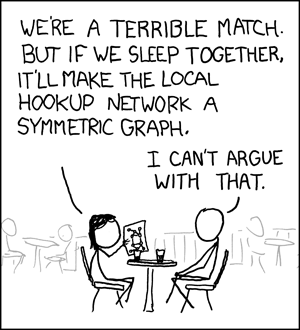
\includegraphics[scale=0.5]{images/xkcd-403.png}
	\end{center}

	\begin{quote}
		\scriptsize{Check it out; I've had sex with someone who's had sex with someone who's written a paper with Paul Erdős!}
	\end{quote}
\end{frame}

\frame{
  \frametitle{Lizenzen}
  \center
  \includegraphics[width=2em]{images/by}
  \includegraphics[width=2em]{images/cc}
  \includegraphics[width=2em]{images/sa}
  \\
  {\tiny

Dieses Werk ist unter einem ``Creative Commons Namensnennung-Weitergabe unter gleichen Bedingungen 3.0 Deutschland``-Lizenzvertrag lizenziert. Um eine Kopie der Lizenz zu erhalten, gehen Sie bitte zu \href{http://creativecommons.org/licenses/by-sa/3.0/de/}{http://creativecommons.org/licenses/by-sa/3.0/de/} oder schreiben Sie an Creative Commons, 171 Second Street, Suite 300, San Francisco, California 94105, USA.\\
  \vspace{1cm}
  Davon ausgenommen sind das Titelbild, welches aus der März-April 2002 Ausgabe von American Scientist erschienen ist und ohne Erlaubnis verwendet wird, sowie das KIT Beamer Theme. Hierfür gelten die Bestimmungen der jeweiligen Urheber.
  \vspace{1cm}
  \\ 
  }
  %Habe hier die Reihenfolge etwas umgestellt, weil die Formatierung bei mir komisch aussah. 
  %Wenn es bei dir anders ist, kannst du es auch wieder zurückändern, dann haben wir unterschiedliche Kompilieroptionen
}

\end{document}
